\documentclass{standalone}
\usepackage{tikz}
\usetikzlibrary{patterns, positioning}


\begin{document}
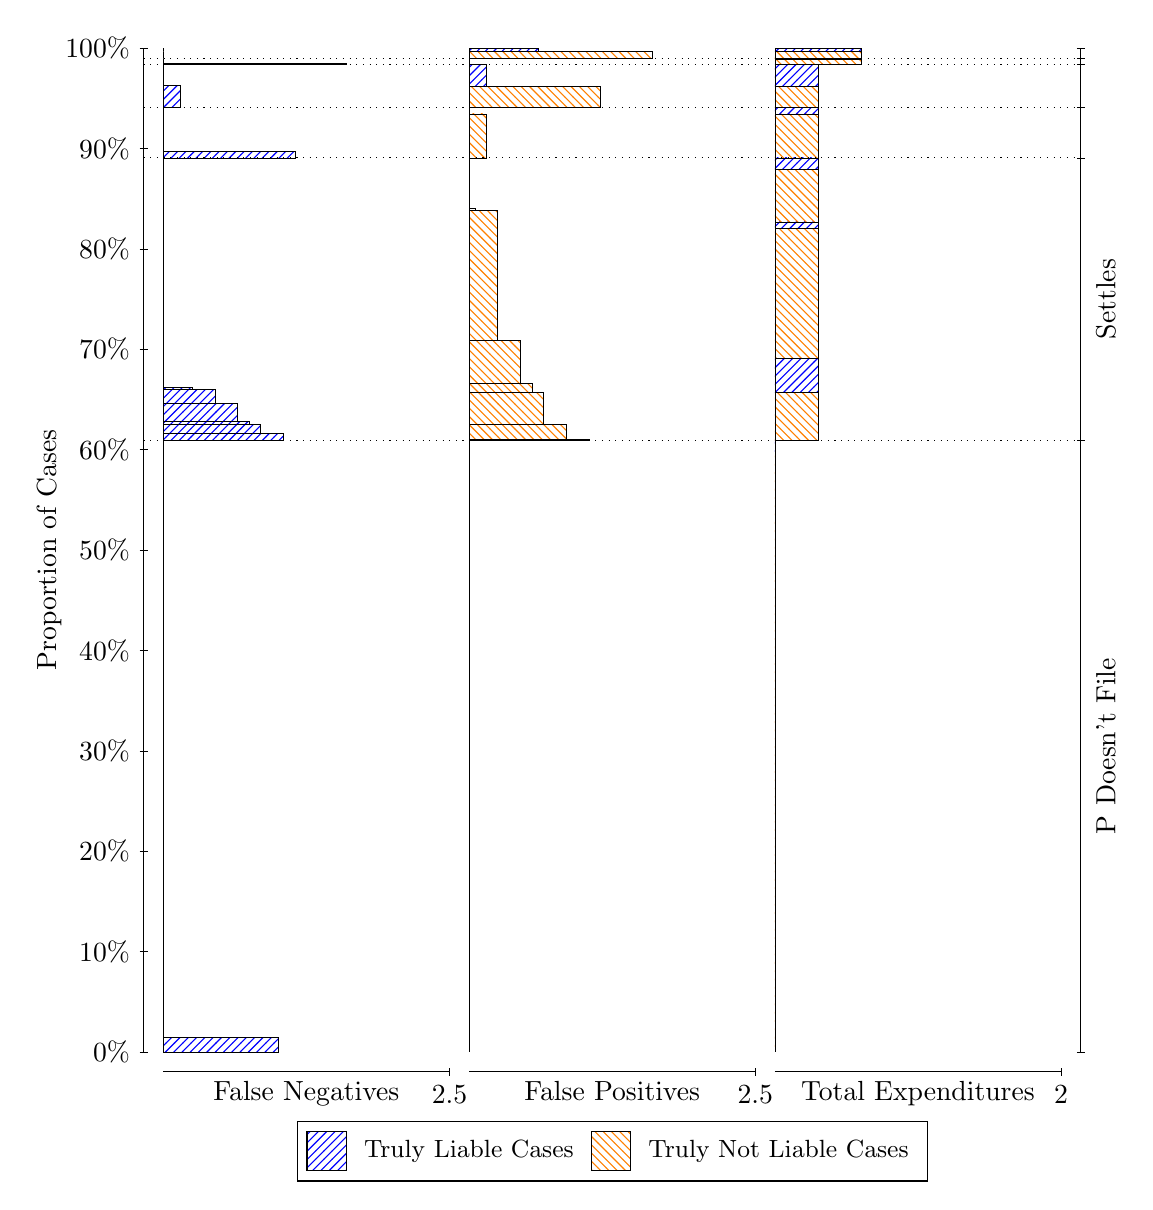
\begin{tikzpicture}
\draw[black, very thin] (1.5,1.75) -- (1.5,14.5);
\node[rotate=90, text=black, anchor=center] at (0.3, 8.125) {Proportion of Cases};
\draw[black, very thin] (1.45,1.75) -- (1.55,1.75);
\node[text=black, anchor=east] at (1.45, 1.75) {0\%};
\draw[black, very thin] (1.45,3.025) -- (1.55,3.025);
\node[text=black, anchor=east] at (1.45, 3.025) {10\%};
\draw[black, very thin] (1.45,4.3) -- (1.55,4.3);
\node[text=black, anchor=east] at (1.45, 4.3) {20\%};
\draw[black, very thin] (1.45,5.575) -- (1.55,5.575);
\node[text=black, anchor=east] at (1.45, 5.575) {30\%};
\draw[black, very thin] (1.45,6.85) -- (1.55,6.85);
\node[text=black, anchor=east] at (1.45, 6.85) {40\%};
\draw[black, very thin] (1.45,8.125) -- (1.55,8.125);
\node[text=black, anchor=east] at (1.45, 8.125) {50\%};
\draw[black, very thin] (1.45,9.4) -- (1.55,9.4);
\node[text=black, anchor=east] at (1.45, 9.4) {60\%};
\draw[black, very thin] (1.45,10.675) -- (1.55,10.675);
\node[text=black, anchor=east] at (1.45, 10.675) {70\%};
\draw[black, very thin] (1.45,11.95) -- (1.55,11.95);
\node[text=black, anchor=east] at (1.45, 11.95) {80\%};
\draw[black, very thin] (1.45,13.225) -- (1.55,13.225);
\node[text=black, anchor=east] at (1.45, 13.225) {90\%};
\draw[black, very thin] (1.45,14.5) -- (1.55,14.5);
\node[text=black, anchor=east] at (1.45, 14.5) {100\%};

\draw[black, very thin] (13.4,1.75) -- (13.4,14.5);
\draw[black, very thin] (13.35,1.75) -- (13.45,1.75);
\node[anchor=west] at (13.35, 1.75) {};
\draw[black, very thin] (13.35,9.519) -- (13.45,9.519);
\node[anchor=west] at (13.35, 9.519) {};
\draw[black, very thin] (13.35,13.106) -- (13.45,13.106);
\node[anchor=west] at (13.35, 13.106) {};
\draw[black, very thin] (13.35,13.746) -- (13.45,13.746);
\node[anchor=west] at (13.35, 13.746) {};
\draw[black, very thin] (13.35,14.292) -- (13.45,14.292);
\node[anchor=west] at (13.35, 14.292) {};
\draw[black, very thin] (13.35,14.37) -- (13.45,14.37);
\node[anchor=west] at (13.35, 14.37) {};
\draw[black, very thin] (13.35,14.5) -- (13.45,14.5);
\node[anchor=west] at (13.35, 14.5) {};

\draw[black, very thin, pattern color=blue, pattern=north east lines] (1.75,1.75) rectangle (3.2033,1.9398);
\draw[black, very thin, pattern color=orange, pattern=north west lines] (1.75,1.9398) rectangle (1.75,9.519);
\draw[black, very thin, pattern color=blue, pattern=north east lines] (1.75,9.519) rectangle (3.276,9.6061);
\draw[black, very thin, pattern color=blue, pattern=north east lines] (1.75,9.6061) rectangle (2.9853,9.7225);
\draw[black, very thin, pattern color=blue, pattern=north east lines] (1.75,9.7225) rectangle (2.84,9.7576);
\draw[black, very thin, pattern color=blue, pattern=north east lines] (1.75,9.7576) rectangle (2.6947,9.9913);
\draw[black, very thin, pattern color=blue, pattern=north east lines] (1.75,9.9913) rectangle (2.404,10.166);
\draw[black, very thin, pattern color=blue, pattern=north east lines] (1.75,10.166) rectangle (2.1133,10.186);
\draw[black, very thin, pattern color=orange, pattern=north west lines] (1.75,10.186) rectangle (1.75,13.106);
\draw[black, very thin, pattern color=blue, pattern=north east lines] (1.75,13.106) rectangle (3.4213,13.189);
\draw[black, very thin, pattern color=orange, pattern=north west lines] (1.75,13.189) rectangle (1.75,13.746);
\draw[black, very thin, pattern color=blue, pattern=north east lines] (1.75,13.746) rectangle (1.968,14.028);
\draw[black, very thin, pattern color=orange, pattern=north west lines] (1.75,14.028) rectangle (1.75,14.292);
\draw[black, very thin, pattern color=blue, pattern=north east lines] (1.75,14.292) rectangle (4.0753,14.302);
\draw[black, very thin, pattern color=orange, pattern=north west lines] (1.75,14.302) rectangle (1.75,14.37);
\draw[black, very thin, pattern color=orange, pattern=north west lines] (1.75,14.37) rectangle (1.75,14.456);
\draw[black, very thin, pattern color=blue, pattern=north east lines] (1.75,14.456) rectangle (1.75,14.5);
\draw[black, very thin, pattern color=orange, pattern=north west lines] (5.6333,1.75) rectangle (5.6333,9.3292);
\draw[black, very thin, pattern color=blue, pattern=north east lines] (5.6333,9.3292) rectangle (5.6333,9.519);
\draw[black, very thin, pattern color=orange, pattern=north west lines] (5.6333,9.519) rectangle (7.1593,9.532);
\draw[black, very thin, pattern color=orange, pattern=north west lines] (5.6333,9.532) rectangle (6.8687,9.7178);
\draw[black, very thin, pattern color=orange, pattern=north west lines] (5.6333,9.7178) rectangle (6.578,10.128);
\draw[black, very thin, pattern color=orange, pattern=north west lines] (5.6333,10.128) rectangle (6.4327,10.239);
\draw[black, very thin, pattern color=orange, pattern=north west lines] (5.6333,10.239) rectangle (6.2873,10.79);
\draw[black, very thin, pattern color=orange, pattern=north west lines] (5.6333,10.79) rectangle (5.9967,12.439);
\draw[black, very thin, pattern color=blue, pattern=north east lines] (5.6333,12.439) rectangle (5.706,12.459);
\draw[black, very thin, pattern color=blue, pattern=north east lines] (5.6333,12.459) rectangle (5.6333,13.106);
\draw[black, very thin, pattern color=orange, pattern=north west lines] (5.6333,13.106) rectangle (5.8513,13.663);
\draw[black, very thin, pattern color=blue, pattern=north east lines] (5.6333,13.663) rectangle (5.6333,13.746);
\draw[black, very thin, pattern color=orange, pattern=north west lines] (5.6333,13.746) rectangle (7.3047,14.01);
\draw[black, very thin, pattern color=blue, pattern=north east lines] (5.6333,14.01) rectangle (5.8513,14.292);
\draw[black, very thin, pattern color=orange, pattern=north west lines] (5.6333,14.292) rectangle (5.6333,14.361);
\draw[black, very thin, pattern color=blue, pattern=north east lines] (5.6333,14.361) rectangle (5.6333,14.37);
\draw[black, very thin, pattern color=orange, pattern=north west lines] (5.6333,14.37) rectangle (7.9587,14.456);
\draw[black, very thin, pattern color=blue, pattern=north east lines] (5.6333,14.456) rectangle (6.5053,14.5);
\draw[black, very thin, pattern color=orange, pattern=north west lines] (9.5167,1.75) rectangle (9.5167,9.3292);
\draw[black, very thin, pattern color=blue, pattern=north east lines] (9.5167,9.3292) rectangle (9.5167,9.519);
\draw[black, very thin, pattern color=orange, pattern=north west lines] (9.5167,9.519) rectangle (10.062,10.128);
\draw[black, very thin, pattern color=blue, pattern=north east lines] (9.5167,10.128) rectangle (10.062,10.556);
\draw[black, very thin, pattern color=orange, pattern=north west lines] (9.5167,10.556) rectangle (10.062,12.205);
\draw[black, very thin, pattern color=blue, pattern=north east lines] (9.5167,12.205) rectangle (10.062,12.293);
\draw[black, very thin, pattern color=orange, pattern=north west lines] (9.5167,12.293) rectangle (10.062,12.955);
\draw[black, very thin, pattern color=blue, pattern=north east lines] (9.5167,12.955) rectangle (10.062,13.106);
\draw[black, very thin, pattern color=orange, pattern=north west lines] (9.5167,13.106) rectangle (10.062,13.663);
\draw[black, very thin, pattern color=blue, pattern=north east lines] (9.5167,13.663) rectangle (10.062,13.746);
\draw[black, very thin, pattern color=orange, pattern=north west lines] (9.5167,13.746) rectangle (10.062,14.01);
\draw[black, very thin, pattern color=blue, pattern=north east lines] (9.5167,14.01) rectangle (10.062,14.292);
\draw[black, very thin, pattern color=orange, pattern=north west lines] (9.5167,14.292) rectangle (10.607,14.361);
\draw[black, very thin, pattern color=blue, pattern=north east lines] (9.5167,14.361) rectangle (10.607,14.37);
\draw[black, very thin, pattern color=orange, pattern=north west lines] (9.5167,14.37) rectangle (10.607,14.456);
\draw[black, very thin, pattern color=blue, pattern=north east lines] (9.5167,14.456) rectangle (10.607,14.5);
\draw[black, dotted] (1.5,9.519) -- (13.4,9.519);
\draw[black, dotted] (1.5,13.106) -- (13.4,13.106);
\draw[black, dotted] (1.5,13.746) -- (13.4,13.746);
\draw[black, dotted] (1.5,14.292) -- (13.4,14.292);
\draw[black, dotted] (1.5,14.37) -- (13.4,14.37);
\draw[black, very thin] (1.75,1.5) -- (5.3833,1.5);
\node[text=black, anchor=north] at (3.5667, 1.5) {False Negatives};
\draw[black, very thin] (5.3833,1.45) -- (5.3833,1.55);
\node[text=black, anchor=north] at (5.3833, 1.45) {2.5};

\draw[black, very thin] (5.6333,1.5) -- (9.2667,1.5);
\node[text=black, anchor=north] at (7.45, 1.5) {False Positives};
\draw[black, very thin] (9.2667,1.45) -- (9.2667,1.55);
\node[text=black, anchor=north] at (9.2667, 1.45) {2.5};

\draw[black, very thin] (9.5167,1.5) -- (13.15,1.5);
\node[text=black, anchor=north] at (11.333, 1.5) {Total Expenditures};
\draw[black, very thin] (13.15,1.45) -- (13.15,1.55);
\node[text=black, anchor=north] at (13.15, 1.45) {2};

\node[text=black, centered, rotate=90] at (13.72, 5.6345) {P Doesn't File};
\node[text=black, centered, rotate=90] at (13.72, 11.312) {Settles};





\draw (7.449999999999999,1.5) node[draw=none] (baseCoordinate) {};
\begin{scope}[align=center]
        \matrix[scale=0.5, draw=black, below=0.5cm of baseCoordinate, nodes={draw}, column sep=0.1cm]{
            \node[rectangle, draw, minimum width=0.5cm, minimum height=0.5cm, pattern color=blue, pattern=north east lines] {}; &
            \node[draw=none, font=\small, text=black] (B) {Truly Liable Cases}; &
            \node[rectangle, draw, minimum width=0.5cm, minimum height=0.5cm, pattern color=orange, pattern=north west lines] {}; &
            \node[draw=none, font=\small, text=black] (B) {Truly Not Liable Cases}; \\
            };
\end{scope}

\end{tikzpicture}
\end{document}